\documentclass[a4paper,12pt]{article}
\usepackage{amsmath}
\usepackage{graphicx}
\usepackage[margin=1in]{geometry}
\usepackage{caption}
\usepackage{authblk}
\usepackage{multirow}
\usepackage{graphicx}
\usepackage{amsmath}
\usepackage{biblatex}
\usepackage{rotating}
\usepackage{ragged2e}
\usepackage{multicol}
\usepackage{float}
\usepackage{algpseudocode}
\usepackage{enumitem}
\usepackage{subcaption}
\usepackage{hyperref}
\hypersetup{
    colorlinks=true,
    linkcolor=blue,
    }
\usepackage[label=corner]{karnaugh-map}
\usepackage[siunitx, RPvoltages]{circuitikz}
\usetikzlibrary{calc}
\usepackage{tikz}
\usetikzlibrary{positioning, shapes, arrows.meta, calc}


\geometry{top=1in, bottom=1in, left=1in, right=1in}

\begin{document}

\begin{center}
    \textbf{CSE 210} \\
    \textbf{Computer Architecture Sessional} \\[.8cm]
    \textbf{Assignment-2: 32-bit Floating Point Adder Simulation} \\[1cm]
    \textbf{Section - C2} \\
    \textbf{Group - } \\[5cm]
\end{center}

\noindent\textbf{Members of the Group:}
\begin{enumerate}
    \item 2105151 - Md.Sani Alam Khan Piyes
    \item 2105152 - Sudip Kumar Saha
    \item 2105167 - Samyo Pramanik
    \item 2105172 - Mezba-Us-Saleheen
\end{enumerate}
\newpage



\section{Introduction}

A computer representation of a real number with a fixed number of digits before and after the decimal point (or radix point in a more general sense) is called a floating point number. A floating point adder is a digital circuit that works with floating point numbers to add and subtract. Numbers that are too large or too small to be accurately represented by integer representations can be represented using this method.

Three fields make up the floating point representation of a number: the sign bit, the exponent field, and the mantissa field. The sign bit represents the sign, either positive or negative. To express a wide range of values, the exponent field permits the significand to be multiplied by a power of the base using a fixed amount of bits in a biased form. The bias needs to be deducted from the stored bits in order to get the real exponent. The fractional portion of the number, or mantissa, is made up of the digits that come after the decimal point. The sign bit, exponent field, and mantissa in this implementation use 1, 9, and 22 bits, respectively. Thus, the exponent bias for our problem would be $2^{9 - 1} - 1 = 256$.

In order to add two numbers, a floating point adder first aligns their decimal points before adding their mantissas. After necessary shifts and related modifications (increment/decrement), the result’s exponent is fixed. Normalization and rounding are performed afterwards. The signs of the two integers being added determine the sign of the outcome.

Applications for floating point adders include financial modeling, computer graphics, and calculations in science and engineering. Because co-processors can be computationally demanding, it is utilized in them to do quick, hardware-accelerated floating point arithmetic. These calculations can be completed far more quickly by a specialized floating point adder than by the main processor. Applications requiring high-precision floating point calculations, such as data analysis and scientific simulations, may find this to be especially crucial.





\section{Problem Specification}

The task involves creating a circuit for a floating point adder that accepts two floating points as inputs, adds their sum, and outputs another floating point. Every floating point will have a length of 32 bits and be represented as follows:
\begin{table}[h]
    \centering
    \begin{tabular}{|c|c|c|}
        \hline
        \textbf{Sign} & \textbf{Exponent} & \textbf{Fraction} \\
        \hline
        1 bit & 9 bits & 22 bits \\
        \hline
    \end{tabular}
    \caption{Problem Specification}
    \label{tab:table1}
\end{table}
\newpage




\section{Description and Circuit Diagram of Modules}
 In order to maintain modularity in the floating point adder design, multiple libraries have
 been built and implemented. Descriptions and usages of the libraries are given below:




\subsection{Processing the Input}


This module (\texttt{InputHandler.circ}) processes the input for further operations in the floating-point adder. It contains:

\begin{itemize}

    \item A circuit that splits the 32-bit floating-point number into an 9-bit exponent and a 20-bit significand,later makes that 20 bit into 32 bit significand.Additionally here is checking if all bit except sign bit is 0,then the significand will be all 0,otherwise with the logic implemented. \texttt{[Input Processor]}.
    \item An exponent differentiator that calculates the difference between the exponents of two inputs \texttt{[Exponent Differentiator]}.
    \item A circuit that determines which input is greater, identifies the greater exponent, calculates the exponent difference, etc., for control decisions \texttt{[Input Handler]}.
\end{itemize}

\begin{figure}[H]
    \centering
    
    \subfloat[Input Processor]{\includegraphics[width=0.3\textwidth]{mezba_image/input_Process .png}}
    \hspace{1cm}
    \subfloat[Exponent Differentiator]{\includegraphics[width=0.3\textwidth]{mezba_image/Exp_process.png}}
    \hspace{1cm}
    \subfloat[Input Handler]{\includegraphics[width=0.3\textwidth]{mezba_image/input_handle.png}}
    \caption{Input Operator Modules}
    \label{fig:input_operator}
\end{figure}




\subsection{Adder Library}
An adder circuit (Significand Adder.circ) has been included in the adder32bit library which performs
 the most crucial part of the FPA, which is to add the significands of the two given input
 f
 loating point numbers.
\begin{figure}[htbp]
    \centering
    \includegraphics[width=1\textwidth]{Significand Adder.png}
    \caption{Significand Adder}
    \label{Significand Adder}
\end{figure}


\subsection{Shifter Library}


\item[\textbf{Left Shifters:}] The left shifters can shift bits by 1, 2, 4, 8, or 16 positions:
        \begin{itemize}
            \item \texttt{1 LeftShift} - Shifts left by 1 bit
            \item \texttt{2 LeftShift} - Shifts left by 2 bits
            \item \texttt{4 LeftShift} - Shifts left by 4 bits
            \item \texttt{8 LeftShift} - Shifts left by 8 bits
            \item \texttt{16 LeftShift} - Shifts left by 16 bits
        \end{itemize}
    
    \item[\textbf{Right Shifters:}] The right shifters can shift bits by 1, 2, 4, 8, or 16 positions:
        \begin{itemize}
            \item \texttt{1 RightShift} - Shifts right by 1 bit
            \item \texttt{2 RightShift} - Shifts right by 2 bits
            \item \texttt{4 RightShift} - Shifts right by 4 bits
            \item \texttt{8 RightShift} - Shifts right by 8 bits
            \item \texttt{16 RightShift} - Shifts right by 16 bits
        \end{itemize}
    
    \item\textbf{Arbitrary Shifters:} These shifters can shift by any number of bits up to 31 bits:
        \begin{itemize}
            \item \texttt{Arbitary LeftShift} - Shifts left by an arbitrary number of bits (up to 31)
            \item \texttt{Arbitary RightShift} - Shifts right by an arbitrary number of bits (up to 31)
        \end{itemize}
    
    \item\textbf{Right Shifter with Empty:} This shifter sets all bits to 0 if the shift amount exceeds 31 bits:
        \begin{itemize}
            \item \texttt{Right Shift With Empty} - Right shifts up to 31 bits, or sets all bits to 0 if more than 31 bits
        \end{itemize}

        

\begin{figure}[H]
    \centering
    % Row 1
    \begin{subfigure}[b]{0.3\textwidth}
        \centering
        \includegraphics[width=\linewidth]{1 bit leftShifter.png}
        \subcaption{1 bit left shifter}
    \end{subfigure}
    \hfill
    \begin{subfigure}[b]{0.3\textwidth}
        \centering
        \includegraphics[width=\linewidth]{2 bit leftShifter.png}
        \subcaption{2 bit left shifter}
    \end{subfigure}
    \hfill
    \begin{subfigure}[b]{0.3\textwidth}
        \centering
        \includegraphics[width=\linewidth]{4 bit leftShifter.png}
        \subcaption{4 bit left shifter}
    \end{subfigure}
    \newline
    \newline
    \vspace{1em}

    % Row 2
    \begin{subfigure}[b]{0.3\textwidth}
        \centering
        \includegraphics[width=\linewidth]{8 bit leftShifter.png}
        \subcaption{8 bit left shifter}
    \end{subfigure}
    \hfill
    \begin{subfigure}[b]{0.3\textwidth}
        \centering
        \includegraphics[width=\linewidth]{16 bit leftShifter.png}
        \subcaption{16 bit left shifter}
    \end{subfigure}
    \hfill
    \begin{subfigure}[b]{0.3\textwidth}
        \centering
        \includegraphics[width=\linewidth]{Arbitary leftShifter.png}
        \subcaption{Arbitary left shifter}
    \end{subfigure}
    \newline
    \newline
    \vspace{1em}

    % Row 3
    \begin{subfigure}[b]{0.3\textwidth}
        \centering
        \includegraphics[width=\linewidth]{1 bit rightShifter.png}
        \subcaption{1 bit right shifter}
    \end{subfigure}
    \hfill
    \begin{subfigure}[b]{0.3\textwidth}
        \centering
        \includegraphics[width=\linewidth]{2 bit righShifter.png}
        \subcaption{2 bit right shifter}
    \end{subfigure}
    \hfill
    \begin{subfigure}[b]{0.3\textwidth}
        \centering
        \includegraphics[width=\linewidth]{4 bit rightShifter.png}
        \subcaption{4 bit right shifter}
    \end{subfigure}
    \newline
    \newline
    \vspace{1em}

    % Row 4
    \begin{subfigure}[b]{0.3\textwidth}
        \centering
        \includegraphics[width=\linewidth]{8 bit rightShifter.png}
        \subcaption{8 bit right shifter}
    \end{subfigure}
    \hfill
    \begin{subfigure}[b]{0.3\textwidth}
        \centering
        \includegraphics[width=\linewidth]{16 bit rightShifter.png}
        \subcaption{16 bit right shifter}
    \end{subfigure}
    \hfill
    \begin{subfigure}[b]{0.3\textwidth}
        \centering
        \includegraphics[width=\linewidth]{Arbitary RightShifter.png}
        \subcaption{Arbitary Right Shifter}
    \end{subfigure}
    \newline
    \newline
    \hfill
    \begin{subfigure}[b]{0.3\textwidth}
        \centering
        \includegraphics[width=\linewidth]{Right_Shifter.png}
        \subcaption{Right Shift with empty}
    \end{subfigure}
    \caption{Shifter Circuits}


\end{figure}

\pagebreak

\subsection{Normalizer Library}



\subsection{Rounding Circuit}
The name of the Module is Rounder.circ. It contains two OR gate,one AND gate and a full Adder and does the rounding of the mantissa.

\begin{figure}[htbp]
    \centering
    \includegraphics[width=1\textwidth]{rounder.png}
    \caption{Rounder Circuit}
    \label{rounder}
\end{figure}


\section{Floating Point Adder}
The last module, called FPA.circ, uses the libraries and other modules to fully create a
 floating point adder. It has the real floating point adder, or circuit FPA. The output processor
 circuit that merges the sign, exponent and significand of the result is also included in this
 module.
 
 \begin{figure}[htbp]
    \centering
    \includegraphics[width=1\textwidth]{FPA.png}
    \caption{The FPA}
    \label{FPA}
\end{figure}

\begin{figure}[htbp]
    \centering
    \includegraphics[width=1\textwidth]{Output.png}
    \caption{Output Processor of the Result}
    \label{Output}
\end{figure}


\section{Flowchart of the Addition/Subtraction Algorithm}


% \begin{figure}[htbp]
%     \centering
%     \includegraphics[width=1\textwidth]{Block Diagram.png}
%     \caption{Flow chart of the addition/substraction algorithm}
%     \label{Block Diagram}
% \end{figure}

\begin{figure}[H]
\centering
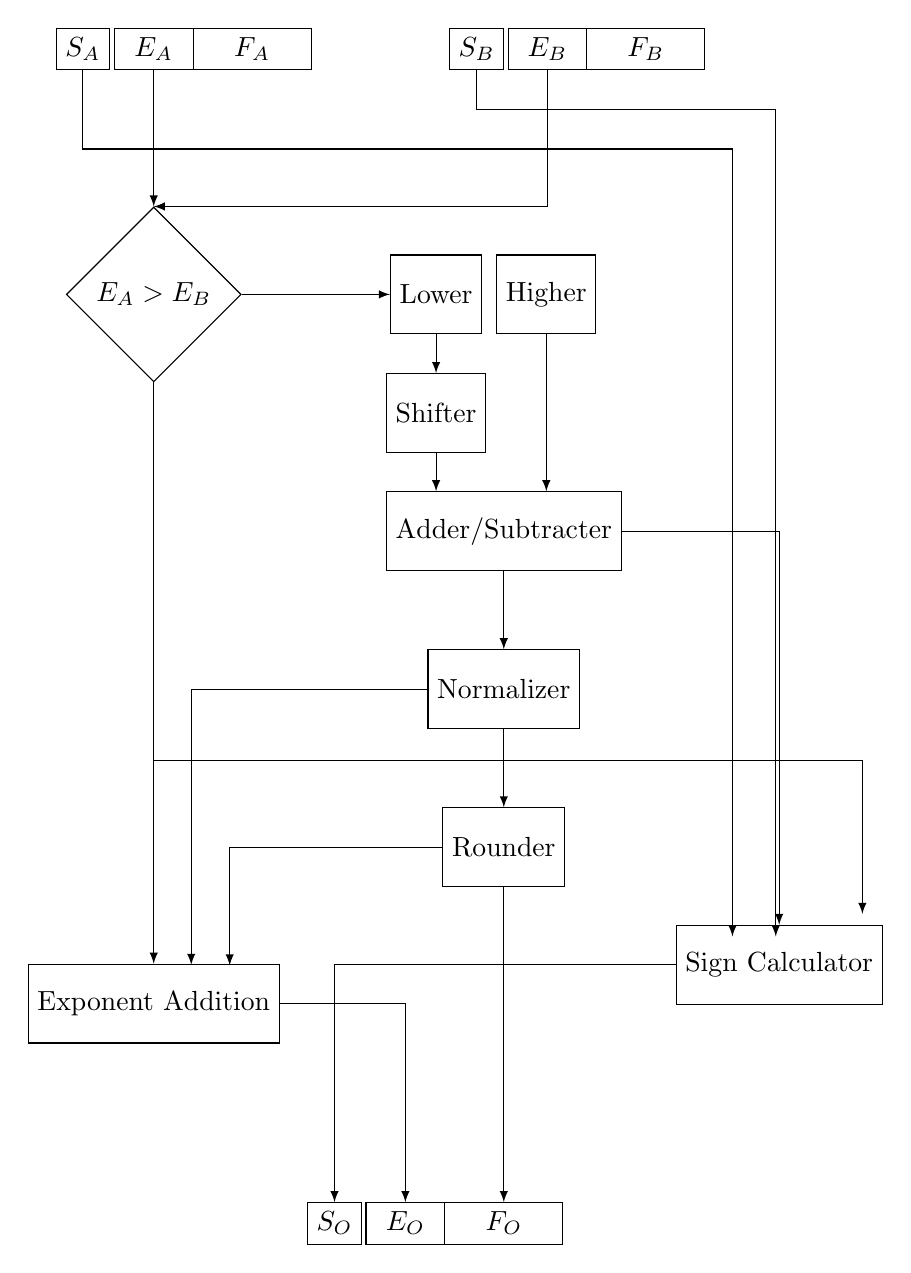
\begin{tikzpicture}
\node[draw,
        minimum width=0.6cm,
        minimum height=0.5cm] (SA) at (0,0) {$S_A$};
\node[draw,
        minimum width=1cm,
        minimum height=0.5cm] (EA) at ($(SA) + (.9, 0)$) {$E_A$};
\node[draw,
        minimum width=1.5cm,
        minimum height=0.5cm] (FA) at ($(EA) + (1.25, 0)$) {$F_A$};

\node[draw,
        minimum width=0.6cm,
        minimum height=0.5cm] (SB) at (5,0) {$S_B$};
\node[draw,
        minimum width=1cm,
        minimum height=0.5cm] (EB) at ($(SB) + (.9, 0)$) {$E_B$};
\node[draw,
        minimum width=1.5cm,
        minimum height=0.5cm] (FB) at ($(EB) + (1.25, 0)$) {$F_B$}; 

\draw [-latex]
    (EA) --++(0, -2) 
    node[diamond, draw, anchor=north] (comp) {$E_A>E_B$};

\draw [-latex]
    (EB) -- (EB |- comp.north) -- (comp.north);

\draw [-latex]
    (comp) --++(3, 0)
    node[draw, 
        minimum width=1cm,
        minimum height=1cm, anchor=west] (low) {Lower};

\node[draw, 
        minimum width=1cm,
        minimum height=1cm] (high) at ($(low) + (1.4, 0)$) {Higher};        

\draw [-latex]
    (low) --++(0, -1)
    node[draw, 
        minimum width=1cm,
        minimum height=1cm, anchor=north] (shift) {Shifter};

\node[draw,
        minimum width=1cm,
        minimum height=1cm,
        anchor=west] (add) at ($(shift.west) + (0, -1.5)$) {Adder/Subtracter};

\draw [-latex] 
    (shift) -- (shift |- add.north);

\draw [-latex]    
    (high) -- (high |- add.north);

\draw [-latex]
    (add) --++(0, -1.5)
     node[draw, 
        minimum width=1cm,
        minimum height=1cm, 
        anchor=north] (norm) {Normalizer};

\draw [-latex]
    (norm) --++(0, -1.5)
     node[draw, 
        minimum width=1cm,
        minimum height=1cm, 
        anchor=north] (Rou) {Rounder};

\draw [-latex]
    (comp) --++(0, -8.5)
     node[draw, 
        minimum width=1cm,
        minimum height=1cm, 
        anchor=north] (Eadd) {Exponent Addition};    

\draw [-latex]
    (Rou.west) --++(-2.7, 0) --++(0, -1.5);

\draw [-latex] 
    (norm.west) --++(-3, 0) --++(0, -3.5);

\draw [-latex]
    (add.east) --++ (2, 0) --++(0, -5) node[draw,
        minimum width=1cm,
        minimum height=1cm, anchor=north] (sign) {Sign Calculator};

\draw [-latex]
    (Rou.south) --++ (0, -4) node[draw,
        minimum width=1.5cm,
        minimum height=0.5cm, anchor=north] (FO) {$F_O$};

\node[draw,
        minimum width=1cm,
        minimum height=0.5cm] (EO) at ($(FO) + (-1.25, 0)$) {$E_O$};                 
        
\node[draw,
        minimum width=0.6cm,
        minimum height=0.5cm] (SO) at ($(EO) + (-0.9, 0)$) {$S_O$};

\draw [-latex]   
    (Eadd.east) -- (EO.north |- Eadd.east) -- (EO.north);

\draw [-latex]
    (SA.south) --++ (0, -1) --++ (8.25, 0) --++ (0, -10);

\draw [-latex]
    (SB.south) --++ (0, -0.5) --++ (3.8, 0) --++ (0, -10.5);

\draw [-latex]
    (comp.south) --++ (0, -4.8) --++ (9.0, 0) --++ (0, -1.95);

\draw [-latex]
    (sign.west) -- (SO.north |- sign.west) -- (SO.north);

\end{tikzpicture}
\caption{Flow chart of the addition/substraction algorithm}
\end{figure}


\section{\large{Comprehensive Design Description}}
\subsection{Comparing the Exponents and Aligning Radix Point}
The radix points need to be lined up in order to add two floating-point values. To align the input with the larger input, this is usually accomplished by moving the input with the smaller exponent to the right. We have computed the difference between the two inputs using a 9-bit subtractor and compared their exponents using a comparator.

\subsection{Shifting}
All shifting operations have been carried out using shifters based on multiplexers. We have employed five 32-bit multiplexers to obtain bit shifts of any arbitrary value up to 31. The multiplexers have the ability to shift 1, 2, 4, 8, and 16 bits in turn. Combining them yields shifts of any length up to 31, as 3f and 3l illustrate. It could take more than 31 shifts to align two fractions, in which case all bits would be 0. Furthermore, the exponent difference ought to be the shifter circuit's input. Thus, after all seven of the higher bits are clear, the lower five bits are used for shifting. The shift amount does not exceed 31($2^{5}-1$) just in that scenario. Otherwise, the fraction will be 0(all bits cleared), which is done in 3m.

\subsection{Normalization}
We used a priority encoder to determine the location of the most significand set bit, which is the leftmost one, in order to normalize and then do an addition operation. To do this, four 8 to 1 priority encoders are employed. 
The result consists of 5 bits ($0-2^{5}-1$), so it can have up to 31 values (from $0_{th} to 31_{th}$). The result's lower three bits are the encoders' output. Using their valid bits, the encoders' upper two bits and outputs are chosen. Other encoders won't be selected and the top two bits will be 00 if the leftmost encoder receives a valid input. Therefore, the decimal range of the integers that are formed is 0 to 7. Likewise, if the second encoder is chosen, the top two bits will be 01; the third and fourth ones will be 10 and 11, respectively. A 4 to 2 priority encoder, whose inputs are the valid bits of the previously stated priority encoders, passes the selection bit of the multiplexer to it. In the event that neither of the priority encoders accepts an input, the fraction is comprised entirely of zeros. This can happen in two cases:
\begin{enumerate}
    \item The result is of the structure $1.00 * 2^{x}$
    \item The result is $0.0$
\end{enumerate}
If two numbers of type $1.00 * 2^{x-1}$ with equal exponents are added, the first instance may manifest. Thus, we can verify if the signs in the two inputs match. If so, we shall proceed with the method and raise the exponent by one. In reality, the outcome is 0 if the signs are opposite. Thus, 0.0 is the output.



\section{Simulator used Along with the Version Number}
logisim-generic-2.7.1 has been used for simulating the floating point adder circuit.


\section{Discussion}
In our project, we aimed to implement a novel design of a Floating Point Adder (FPA). Rather than designing the entire circuit from scratch, we opted for a modular approach, building separate components first and then integrating them to create a functional circuit. This strategy not only simplified the process but also allowed us to distribute the workload effectively.
\newline
\\
We encountered several challenges along the way. The first significant challenge was designing a shifter capable of shifting by any arbitrary amount. To achieve this, we combined 1, 2, 4, 8, and 16-bit shifters in a serial configuration, where each shifter corresponded to one of the bits in the shift amount.\\
\newline
The second challenge was handling negative numbers. We found that the result depended on the signs and relative magnitudes of the inputs. This situation created four possible cases, which we addressed using a combination of adders, subtractors, complementers, XOR gates, and multiplexers.\\
\newline
A third challenge involved accounting for overflow and underflow. We chose not to reserve a separate bit to track overflow or the sign of the result, as discussed . By avoiding the need for an additional bit, we were able to enhance the precision of our implementation by two digits. Instead, we used the carry-out from the adder to manage overflow.\\
\newline
To ensure a minimal yet fully functional design, we used a combination of built-in circuits from the Logisim library and our own custom circuits.\\
\newline
Overall, designing and implementing the floating-point adder was a rewarding experience that deepened our understanding of its inner workings.



\end{document}